\documentclass[aspectratio=169,11pt]{beamer}

\usepackage[T1]{fontenc}
\usepackage[utf8]{inputenc}
\usepackage[english]{babel}
\usepackage{lmodern}
\usepackage{tikz}
\usepackage{qrcode}
\usepackage{fontawesome5}
\usepackage{booktabs}
\usepackage{array}
\newcolumntype{L}[1]{>{\raggedright\arraybackslash}p{#1}}
\usepackage{listings}
\usetikzlibrary{arrows.meta, positioning, shapes.geometric, fit, calc}

% ---------- look ----------
\definecolor{cobgold}{HTML}{B8860B}
\definecolor{cobblue}{HTML}{1F4E79}
\definecolor{cobgrey}{HTML}{555555}
\definecolor{cobgreen}{HTML}{2E7D32}
\definecolor{cobred}{HTML}{B3261E}

\usetheme{default}
\usecolortheme{default}
\setbeamercolor{structure}{fg=cobblue}
\setbeamercolor{title}{fg=cobblue}
\setbeamercolor{frametitle}{fg=cobblue}
\setbeamercolor{block title}{bg=cobblue!12, fg=cobblue}
\setbeamercolor{block body}{bg=cobblue!4}
\setbeamercolor{block title alerted}{bg=cobgold!20, fg=black}
\setbeamercolor{block body alerted}{bg=cobgold!8}
\setbeamercolor{block title example}{bg=cobgreen!15, fg=black}
\setbeamercolor{block body example}{bg=cobgreen!5}
\setbeamertemplate{navigation symbols}{}
\setbeamertemplate{itemize items}[circle]
\setbeamerfont{frametitle}{series=\bfseries, size=\Large}
\setbeamertemplate{footline}{%
  \hfill\usebeamercolor[fg]{footline}\scriptsize\color{cobgrey}%
  CoB to KiCad\quad\insertframenumber/\inserttotalframenumber\hspace{1em}\vspace{0.6em}}

\lstdefinelanguage{cobshell}{morecomment=[l]{\#}}
\lstset{basicstyle=\ttfamily\scriptsize, columns=fullflexible, keepspaces=true,
  frame=single, rulecolor=\color{cobblue!40}, backgroundcolor=\color{cobblue!3}}

\newcommand{\xhslogo}{\raisebox{-0.2ex}{
\includegraphics[height=1.3em]{images/xiaohongshu.png}}}
\newcommand{\halves}[2]{\parbox[t][3.3cm][s]{\linewidth}{\raggedright #1\vfill\raggedright\footnotesize #2}}
\newsavebox{\stackbox}
\newlength{\stackh}
\newlength{\stackw}
\newcommand{\hl}[1]{{\color{cobgold}\textbf{#1}}}

% ---------- metadata ----------
\title{From Bare Die to Bonded Board:\\Chip-on-Board Meets KiCad}
\subtitle{Describe the chip once, generate the rest}
\author{Stephan Bökelmann}
\institute{\texttt{maxclerkwell.tech}}
\date{\today}

\begin{document}

% ======================================================================
\begin{frame}[plain]
  \titlepage
\end{frame}

% ======================================================================
\begin{frame}{Chip design has opened up}
  \small
  \begin{columns}[T,onlytextwidth]
    \column{0.225\textwidth}
      \begin{block}{More open}
        \halves{Open PDKs and open tools: \textbf{OpenROAD}, Yosys, KLayout, Magic, ngspice.}
               {Open PDKs: \textbf{Tim Ansell}}
      \end{block}
    \column{0.225\textwidth}
      \begin{block}{More accessible}
        \halves{Courses from zero to taped-out silicon.}
               {\textbf{Matthew Venn}: \textbf{Tiny Tapeout} and his courses}
      \end{block}
    \column{0.225\textwidth}
      \begin{block}{More affordable}
        \halves{Real silicon, real dies, from shared shuttle runs.}
               {\textbf{wafer.space}, founded by \textbf{Tim Ansell}}
      \end{block}
    \column{0.225\textwidth}
      \begin{block}{More hackable}
        \halves{Chips made in a garage with homebrew equipment.}
               {\textbf{Sam Zeloof} and the \textbf{Hackerfab} community}
      \end{block}
  \end{columns}
  \vfill
  \begin{center}
    \Large Designing a chip is no longer the hard part.\\
    \color{cobgrey}\normalsize Getting the bare dies onto a board is.
  \end{center}
  \vfill
\end{frame}

% ======================================================================
\begin{frame}{What are ICs, and what can you describe?}
  \centering
  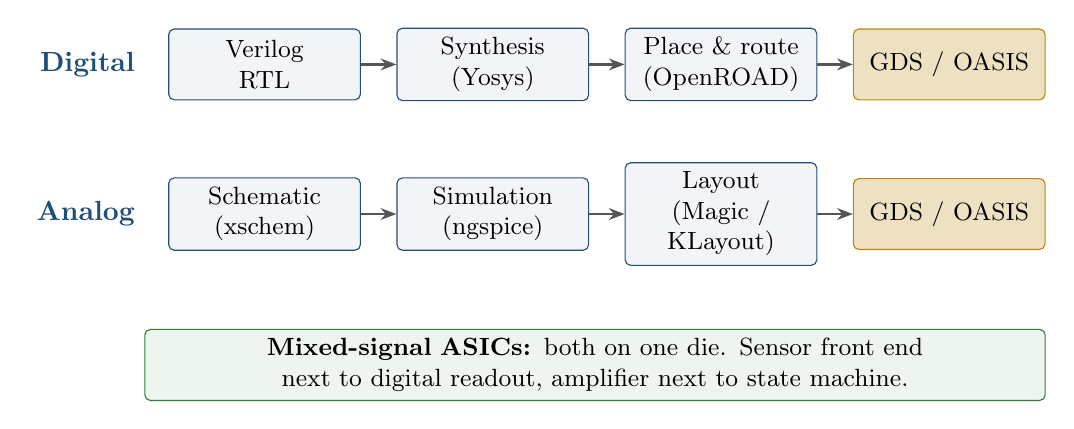
\begin{tikzpicture}[
      box/.style={draw=cobblue, rounded corners=2pt, fill=cobblue!6, align=center,
                  minimum height=0.9cm, text width=2.2cm, font=\small},
      lane/.style={font=\bfseries\color{cobblue}, anchor=east},
      arr/.style={-{Stealth[length=2mm]}, thick, color=cobgrey},
      node distance=0.45cm]
    % digital
    \node[lane] (dl) at (0,1.9) {Digital};
    \node[box, right=0.3cm of dl] (v) {Verilog\\RTL};
    \node[box, right=of v] (syn) {Synthesis\\(Yosys)};
    \node[box, right=of syn] (pnr) {Place \& route\\(OpenROAD)};
    \node[box, right=of pnr, fill=cobgold!25, draw=cobgold] (gds1) {GDS / OASIS};
    \draw[arr] (v)--(syn); \draw[arr] (syn)--(pnr); \draw[arr] (pnr)--(gds1);
    % analog
    \node[lane] (al) at (0,0) {Analog};
    \node[box, right=0.3cm of al] (xs) {Schematic\\(xschem)};
    \node[box, right=of xs] (sim) {Simulation\\(ngspice)};
    \node[box, right=of sim] (lay) {Layout\\(Magic / KLayout)};
    \node[box, right=of lay, fill=cobgold!25, draw=cobgold] (gds2) {GDS / OASIS};
    \draw[arr] (xs)--(sim); \draw[arr] (sim)--(lay); \draw[arr] (lay)--(gds2);
    % mixed
    \node[draw=cobgreen, fill=cobgreen!8, rounded corners=2pt, text width=11.2cm, align=center,
          below=0.8cm of lay, xshift=-1.6cm, font=\small]
      {\textbf{Mixed-signal ASICs:} both on one die. Sensor front end next to digital readout,
       amplifier next to state machine.};
  \end{tikzpicture}
  \vfill
  \small Every path ends in the same artefact: \hl{a layout file}. That is where the physical truth lives.
\end{frame}

% ======================================================================
\begin{frame}{What does it take to characterize an ASIC?}
  \centering
  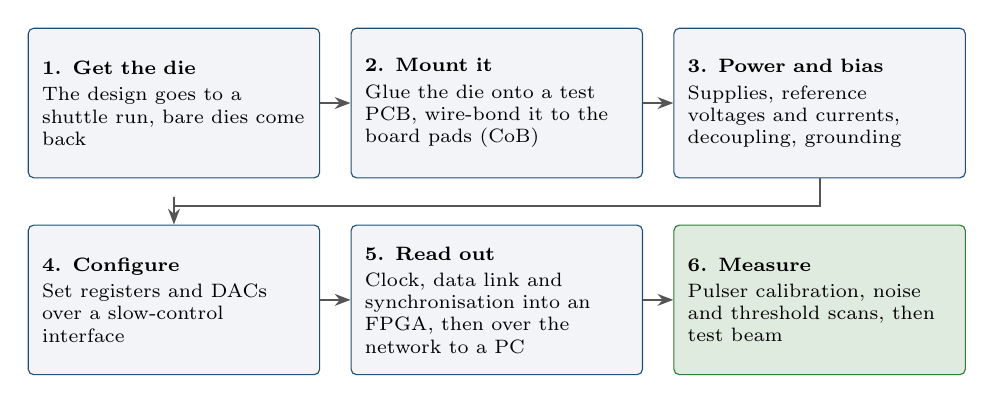
\begin{tikzpicture}[
      pstep/.style={draw=cobblue, rounded corners=2pt, fill=cobblue!6, align=left,
                   minimum height=1.9cm, text width=3.35cm, font=\scriptsize, inner sep=5pt, execute at begin node={\hyphenpenalty=10000\relax}},
      plast/.style={pstep, fill=cobgreen!15, draw=cobgreen},
      arr/.style={-{Stealth[length=2mm]}, thick, color=cobgrey}]
    \node[pstep] (a) at (0,0) {\textbf{1. Get the die}\\[0.2em] The design goes to a shuttle run, bare dies come back};
    \node[pstep] (b) at (4.1,0) {\textbf{2. Mount it}\\[0.2em] Glue the die onto a test PCB, wire-bond it to the board pads (CoB)};
    \node[pstep] (c) at (8.2,0) {\textbf{3. Power and bias}\\[0.2em] Supplies, reference voltages and currents, decoupling, grounding};
    \node[pstep] (d) at (0,-2.5) {\textbf{4. Configure}\\[0.2em] Set registers and DACs over a slow-control interface};
    \node[pstep] (e) at (4.1,-2.5) {\textbf{5. Read out}\\[0.2em] Clock, data link and synchronisation into an FPGA, then over the network to a PC};
    \node[plast] (f) at (8.2,-2.5) {\textbf{6. Measure}\\[0.2em] Pulser calibration, noise and threshold scans, then test beam};
    \draw[arr] (a)--(b); \draw[arr] (b)--(c);
    \draw[arr] (c.south) -- ++(0,-0.35) -| ($(d.north)+(0,0.35)$) -- (d.north);
    \draw[arr] (d)--(e); \draw[arr] (e)--(f);
  \end{tikzpicture}
  \vfill
  \small Every step has to work at the same time before a measurement means anything.
\end{frame}

% ======================================================================
\begin{frame}{Terminology (1): from layout to die}
  \begin{columns}[T]
    \column{0.58\textwidth}
      \footnotesize
      \begin{itemize}\setlength\itemsep{0.35em}
        \item \textbf{GDS / OASIS}: layout file formats with polygons per layer, text labels and nested cells. The truth about the geometry.
        \item \textbf{PDK}: process design kit, the foundry's rules, layer map and cells for one manufacturing process.
        \item \textbf{Shuttle run (MPW)}: many projects share one reticle and one wafer run, so the cost is split.
        \item \textbf{Reticle}: the exposure field of the lithography step. A shuttle reticle holds many projects.
        \item \textbf{Wafer, dicing}: the reticle is exposed many times onto a silicon wafer, then the wafer is sawn apart.
        \item \textbf{Die}: one diced piece of silicon, your chip, bare, without any housing.
      \end{itemize}
    \column{0.38\textwidth}
      \centering
      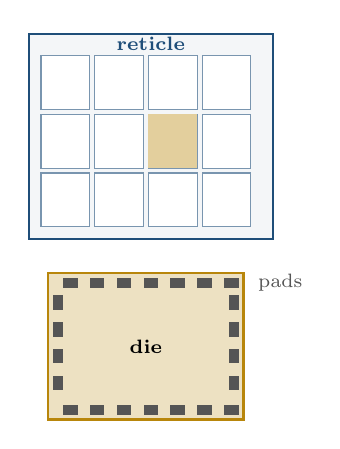
\begin{tikzpicture}[scale=0.62]
        % reticle
        \draw[thick, cobblue, fill=cobblue!5] (0,0) rectangle (5,4.2);
        \foreach \x in {0,1,2,3} \foreach \y in {0,1,2} {
          \draw[cobblue!60, fill=white] (0.25+1.1*\x, 0.25+1.2*\y) rectangle ++(1,1.1);
        }
        \fill[cobgold!40] (0.25+1.1*2, 0.25+1.2*1) rectangle ++(1,1.1);
        \node[font=\scriptsize\bfseries, color=cobblue] at (2.5,4.0) {reticle};
        % zoom on die
        \begin{scope}[shift={(0.4,-3.7)}]
          \draw[thick, cobgold, fill=cobgold!25] (0,0) rectangle (4,3);
          \foreach \i in {0,...,6} {
            \fill[cobgrey] (0.3+0.55*\i,2.7) rectangle ++(0.3,0.2);
            \fill[cobgrey] (0.3+0.55*\i,0.1) rectangle ++(0.3,0.2);
          }
          \foreach \i in {0,...,3} {
            \fill[cobgrey] (0.1,0.6+0.55*\i) rectangle ++(0.2,0.3);
            \fill[cobgrey] (3.7,0.6+0.55*\i) rectangle ++(0.2,0.3);
          }
          \node[font=\scriptsize\bfseries] at (2,1.5) {die};
          \node[font=\scriptsize, color=cobgrey, anchor=west] at (4.1,2.8) {pads};
        \end{scope}
      \end{tikzpicture}
  \end{columns}
\end{frame}

% ======================================================================
\begin{frame}{Terminology (2): pads, wires and the board}
  \footnotesize
  \begin{columns}[T]
    \column{0.5\textwidth}
      \begin{itemize}\setlength\itemsep{0.35em}
        \item \textbf{Metallization}: the top metal layers. They define what a wire can be bonded to and which wire material, force and temperature work.
        \item \textbf{Passivation}: the protective layer over the chip. Where it is opened, the metal is free.
        \item \textbf{Pad}: an opening in the passivation where the die talks to the outside world.
        \item \textbf{Bond finger, bond target}: board copper where the wire lands, and the exact landing point on it.
        \item \textbf{Land pattern, footprint}: the copper pattern on the PCB. In CoB it is new for every chip iteration.
        \item \textbf{Die attach}: gluing the die onto the board, with a conductive or an insulating adhesive.
      \end{itemize}
    \column{0.46\textwidth}
      \begin{block}{Ways to connect die and board}
        \begin{itemize}\setlength\itemsep{0.15em}
          \item \textbf{Wire bonding}: thin wire from die pad to board pad, wedge or ball
          \item \textbf{Flip-chip}: die turned face down, bumps on the pads touch the board pads directly, no wires
          \item \textbf{TAB} (tape automated bonding): metal traces on a flexible tape connect die and board
          \item \textbf{FOPLP} (fan-out panel-level packaging): dies embedded in a panel, thin redistribution layers fan the pads out, no wires
        \end{itemize}
      \end{block}
      {\scriptsize\color{cobgrey} open.cob.json starts with wire bonding and leaves room for the other techniques.}
  \end{columns}
\end{frame}

% ======================================================================
\begin{frame}{Packaged vs.\ Chip-on-Board}
  \begin{columns}[T]
    \column{0.48\textwidth}
      \begin{block}{Packaged}
        \centering
        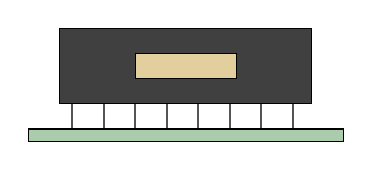
\begin{tikzpicture}[scale=0.8]
          \draw[fill=black!75] (0,0.4) rectangle (4,1.6);
          \draw[fill=cobgold!40] (1.2,0.8) rectangle (2.8,1.2);
          \foreach \x in {0.2,0.7,...,3.7} {\draw[thick, cobgrey] (\x,0.4)--(\x,0);}
          \draw[fill=cobgreen!40] (-0.5,-0.2) rectangle (4.5,0);
        \end{tikzpicture}\\[0.4em]
        \raggedright
        \begin{itemize}\setlength\itemsep{0.2em}
          \item Standard footprint (QFN, QFP, \dots), solder it and done
          \item Package costs money and lead time
          \item Package adds inductance and size
          \item The pinout is fixed by the package
        \end{itemize}
      \end{block}
    \column{0.48\textwidth}
      \begin{alertblock}{Chip-on-Board}
        \centering
        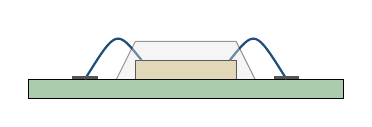
\begin{tikzpicture}[scale=0.8]
          \draw[fill=cobgreen!40] (-0.5,0) rectangle (4.5,0.3);
          \draw[fill=cobgold!40] (1.2,0.3) rectangle (2.8,0.6);
          \foreach \x/\y in {1.4/0.5, 1.9/0.5, 2.4/0.5} {}
          \draw[thick, cobblue] (1.3,0.6) .. controls (0.9,1.1) .. (0.4,0.3);
          \draw[thick, cobblue] (2.7,0.6) .. controls (3.1,1.1) .. (3.6,0.3);
          \fill[cobgrey] (0.2,0.3) rectangle (0.6,0.35);
          \fill[cobgrey] (3.4,0.3) rectangle (3.8,0.35);
          \draw[fill=black!10, opacity=0.4] (0.9,0.3) -- (1.2,0.9) -- (2.8,0.9) -- (3.1,0.3);
        \end{tikzpicture}\\[0.4em]
        \raggedright
        \begin{itemize}\setlength\itemsep{0.2em}
          \item Bare die first glued onto the PCB, then wires bonded to board pads
          \item No package: cheaper, smaller, shorter wires
          \item Direct access to special pads, probe points, sensors
          \item \textbf{But: no standard footprint}. You design it for each chip.
        \end{itemize}
      \end{alertblock}
  \end{columns}
  \vfill
  \centering\small\color{cobgrey} A 2~mm die on a PCB: the wires fan out from the chip edge to bond fingers.
\end{frame}

% ======================================================================
\begin{frame}{Four ways to connect die and board}
  \small
  \begin{columns}[T]
    \column{0.49\textwidth}
      \centering
      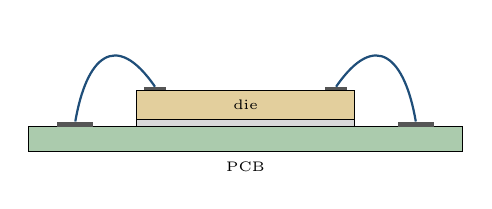
\begin{tikzpicture}[scale=0.92]
        \draw[fill=cobgreen!40] (0,0) rectangle (6,0.35);
        \fill[cobgrey] (0.4,0.35) rectangle (0.9,0.42); \fill[cobgrey] (5.1,0.35) rectangle (5.6,0.42);
        \draw[fill=black!15] (1.5,0.35) rectangle (4.5,0.45);
        \draw[fill=cobgold!40] (1.5,0.45) rectangle (4.5,0.85);
        \fill[cobgrey] (1.6,0.85) rectangle (1.9,0.9); \fill[cobgrey] (4.1,0.85) rectangle (4.4,0.9);
        \draw[thick, cobblue] (1.75,0.9) .. controls (1.2,1.7) and (0.8,1.3) .. (0.65,0.42);
        \draw[thick, cobblue] (4.25,0.9) .. controls (4.8,1.7) and (5.2,1.3) .. (5.35,0.42);
        \node[font=\tiny] at (3,0.65) {die};
        \node[font=\tiny, anchor=north] at (3,0.0) {PCB};
      \end{tikzpicture}\\[0.1em]
      \textbf{Wire bonding}: die glued to the board first (die attach), then thin wires from die pads to board pads\\[1.4em]
      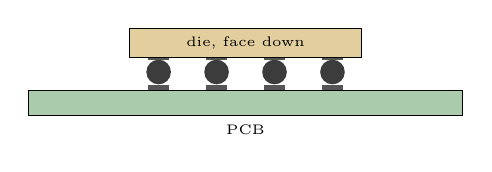
\begin{tikzpicture}[scale=0.92]
        \draw[fill=cobgreen!40] (0,0) rectangle (6,0.35);
        \foreach \x in {1.8,2.6,3.4,4.2} {
          \fill[cobgrey] (\x-0.15,0.35) rectangle (\x+0.15,0.42);
          \fill[cobgrey!70!black] (\x,0.6) circle (0.17);
          \fill[cobgrey] (\x-0.15,0.77) rectangle (\x+0.15,0.8);
        }
        \draw[fill=cobgold!40] (1.4,0.8) rectangle (4.6,1.2);
        \node[font=\tiny] at (3,1.0) {die, face down};
        \node[font=\tiny, anchor=north] at (3,0.0) {PCB};
      \end{tikzpicture}\\[0.1em]
      \textbf{Flip-chip}: die face down, solder bumps touch the board pads, no wires
    \column{0.49\textwidth}
      \centering
      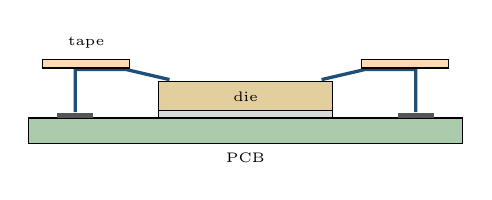
\begin{tikzpicture}[scale=0.92]
        \draw[fill=cobgreen!40] (0,0) rectangle (6,0.35);
        \fill[cobgrey] (0.4,0.35) rectangle (0.9,0.42); \fill[cobgrey] (5.1,0.35) rectangle (5.6,0.42);
        \draw[fill=black!15] (1.8,0.35) rectangle (4.2,0.45);
        \draw[fill=cobgold!40] (1.8,0.45) rectangle (4.2,0.85);
        \draw[very thick, cobblue] (1.95,0.88) -- (1.35,1.02) -- (0.65,1.02) -- (0.65,0.43);
        \draw[very thick, cobblue] (4.05,0.88) -- (4.65,1.02) -- (5.35,1.02) -- (5.35,0.43);
        \draw[fill=orange!30] (0.2,1.04) rectangle (1.4,1.16);
        \draw[fill=orange!30] (4.6,1.04) rectangle (5.8,1.16);
        \node[font=\tiny] at (3,0.65) {die};
        \node[font=\tiny, anchor=south] at (0.8,1.18) {tape};
        \node[font=\tiny, anchor=north] at (3,0.0) {PCB};
      \end{tikzpicture}\\[0.1em]
      \textbf{TAB} (tape automated bonding): metal leads on a flexible tape connect die and board\\[1.4em]
      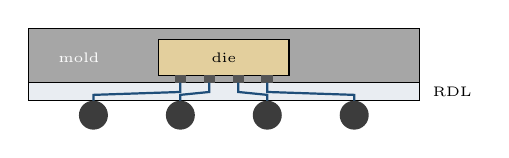
\begin{tikzpicture}[scale=0.92]
        \draw[fill=black!35] (0.3,0.85) rectangle (5.7,1.6);
        \draw[fill=cobgold!40] (2.1,0.95) rectangle (3.9,1.45);
        \draw[fill=cobblue!10] (0.3,0.6) rectangle (5.7,0.85);
        \foreach \x/\b in {2.4/1.2, 2.8/2.4, 3.2/3.6, 3.6/4.8} {
          \fill[cobgrey] (\x-0.08,0.85) rectangle (\x+0.08,0.95);
          \draw[cobblue, thick] (\x,0.85) -- (\x,0.72) -- (\b,0.68) -- (\b,0.58);
          \fill[cobgrey!70!black] (\b,0.4) circle (0.2);
        }
        \node[font=\tiny, color=white] at (1.0,1.2) {mold};
        \node[font=\tiny] at (3,1.2) {die};
        \node[font=\tiny, anchor=west] at (5.75,0.72) {RDL};
      \end{tikzpicture}\\[0.1em]
      \textbf{FOPLP}: dies embedded in a panel, redistribution layers fan the pads out to solder balls
  \end{columns}
  \vfill
  {\scriptsize\color{cobgrey} Wire bonding in detail: my talk \textit{Poor Man's Introduction to Wire-Bonding}, KiCon Europe 2025 (Bochum) and KiCon Asia 2025 (Shenzhen).}
\end{frame}

% ======================================================================
\begin{frame}{What I did so far}
  \begin{columns}[T,onlytextwidth]
    \column{0.62\textwidth}
      \begin{itemize}\setlength\itemsep{0.8em}
        \item Characterizing \textbf{mixed-signal ASICs} of the \textbf{HVMAPS} type\\
          {\small High-voltage monolithic active pixel sensors for particle detectors}
        \item Sensor, analog front end and digital readout on a single die
        \item Many chip iterations, each one bonded to a new board
        \item Worked at \textbf{Ruhr University Bochum}\\
          {\small Chair of Experimental Physics I}
        \item Now transferring to \textbf{FAIR}\\
          {\small Facility for Antiproton and Ion Research, Darmstadt}
      \end{itemize}
    \column{0.34\textwidth}
      \centering
      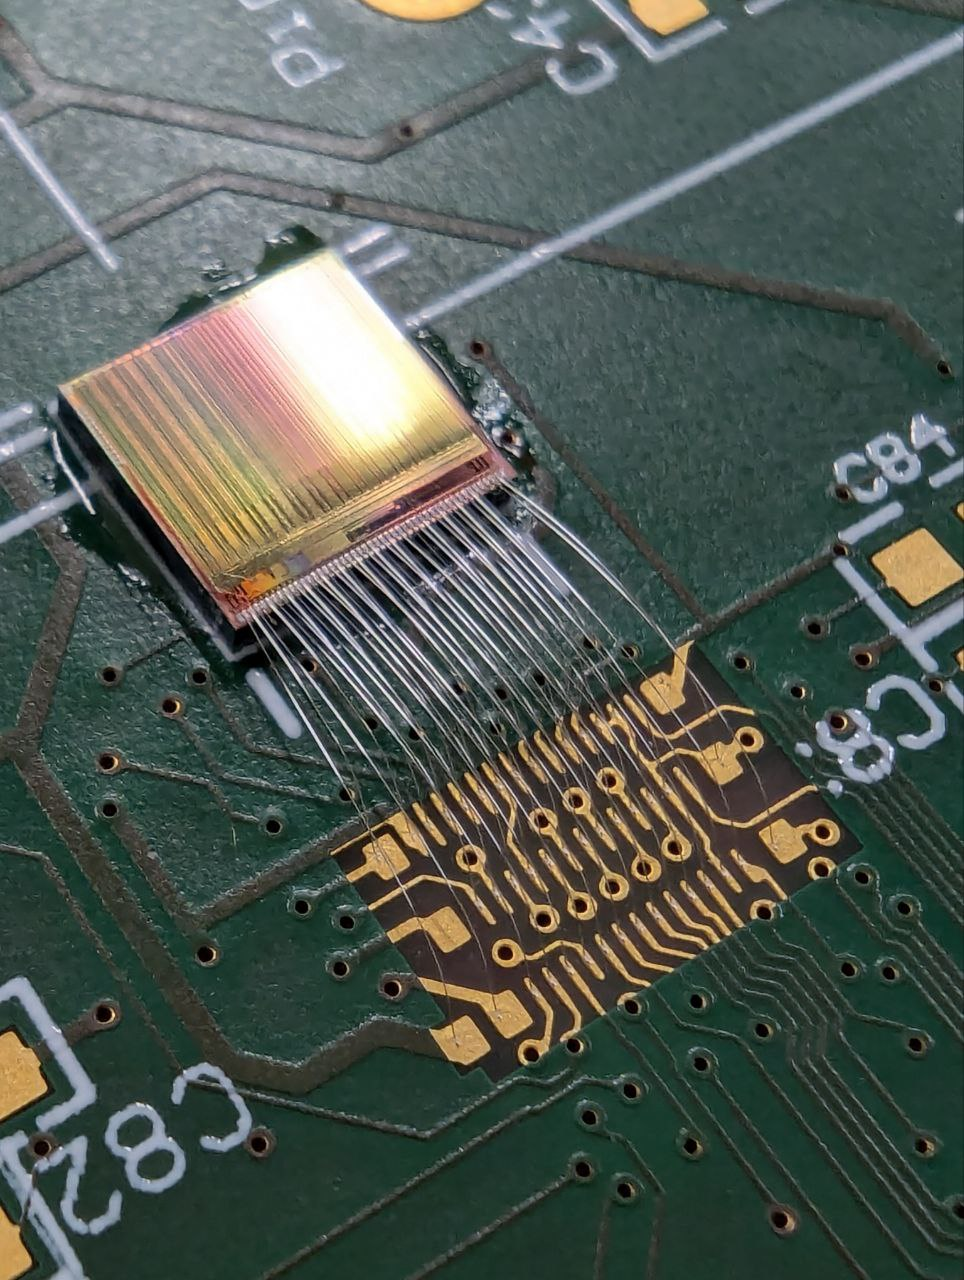
\includegraphics[height=0.62\textheight]{images/die-on-board.jpg}\\[0.2em]
      {\scriptsize\color{cobgrey} A bare die glued onto a PCB, wires fanning out to bond fingers}
  \end{columns}
\end{frame}

% ======================================================================
\begin{frame}{How do we make a PCB for CoB?}
  \begin{columns}[T]
    \column{0.52\textwidth}
      \footnotesize
      \begin{itemize}\setlength\itemsep{0.15em}
        \item Which chip pad goes to which board pad?
        \item How long may a wire become?
        \item Where do cutouts, keepouts and courtyards go?
        \item \textbf{Pad layout}: pitch, angle, stagger, ground bonds, probe pads
        \item \textbf{New chip iteration = new footprint}. Every time.
      \end{itemize}
      \vspace{0.1em}
      \begin{alertblock}{Bottom line}
        There is no canonical exchange format for chip-to-PCB integration yet.
      \end{alertblock}
      \begin{exampleblock}{Silver lining}
        All the data is already in the \textbf{GDS / OASIS} file.
      \end{exampleblock}
    \column{0.44\textwidth}
      \centering
      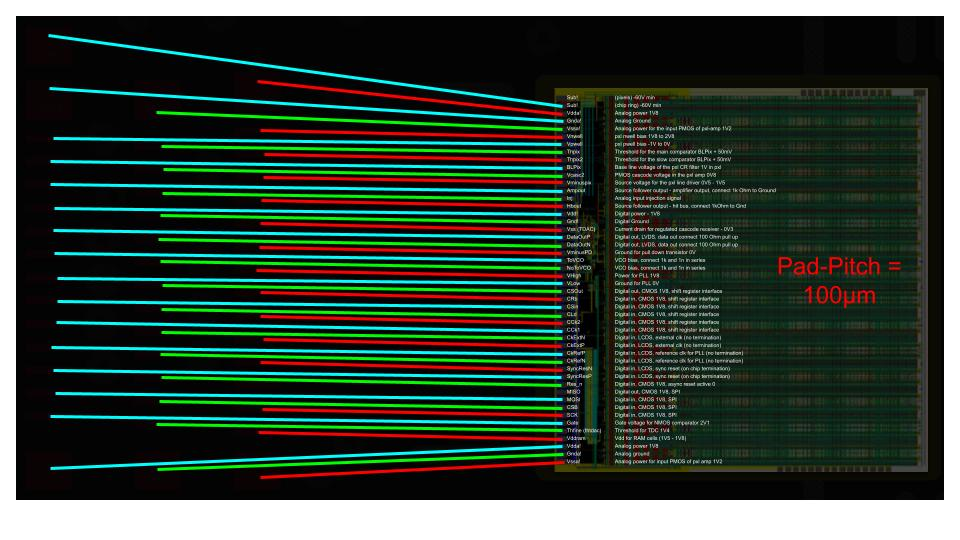
\includegraphics[width=\textwidth]{images/legacy-bonding-plan-example.jpg}\\[0.2em]
      {\scriptsize\color{cobgrey} Today: a bonding plan as a presentation slide.\\
       Not machine-readable, drifts out of sync.}
  \end{columns}
\end{frame}

% ======================================================================
\begin{frame}{The current difficulties}
  \small
  \begin{columns}[T]
    \column{0.485\textwidth}
      \begin{alertblock}{1. The data is scattered}
        Pad positions in the GDS, names and types in the schematic, metal and wire limits in process documents, the bonding plan on a slide. Nothing is machine-readable, the copies drift apart.
      \end{alertblock}
      \begin{alertblock}{2. Chicken and egg}
        Wire length and angle depend on the land pattern, but the land pattern is exactly what you are trying to design.
      \end{alertblock}
    \column{0.485\textwidth}
      \begin{alertblock}{3. New chip, new footprint}
        Every chip iteration needs its own land pattern, drawn by hand, pad by pad.
      \end{alertblock}
      \begin{alertblock}{4. Tolerances stay invisible}
        A die placed 50 to 100 $\mu$m off moves every wire landing point. In a drawing or a slide nobody can check this automatically.
      \end{alertblock}
  \end{columns}
  \vfill
  \begin{center}
    Each one is a manual, undocumented step.\\
    \color{cobgrey}\footnotesize The goal: make them explicit, in one file.
  \end{center}
\end{frame}

% ======================================================================
\begin{frame}{Requirements for an exchange format}
  \footnotesize
  \vspace{0.3em}
  \renewcommand{\arraystretch}{1.0}
  \begin{tabular}{@{}L{3.3cm}L{7.2cm}c@{}}
    \toprule
    \textbf{Requirement} & \textbf{In practice} & \textbf{Fixes}\\
    \midrule
    One file per die & One UUID, one source of truth for chip, board and wires & 1\\
    Open and machine-readable & Plain JSON, readable by people, diffable in git, no tool lock-in & 1\\
    Honest about gaps & \texttt{"none"} means deliberately absent, \texttt{"unspecified"} means unknown. Nothing is guessed & 1\\
    Explicit tolerances & Nominal $\pm$ tolerance or ranges, so the die placement can widen every wire landing & 4\\
    Reusable land patterns & Shapes from a catalog, placed by reference, scaled and rotated & 3\\
    Derive, do not redraw & Footprint, symbol, bond parameters and tests come from the same file & 2, 3\\
    Usable in stages & The chip designer delivers a die-only file, the PCB designer adds the rest & 2\\
    Open to extension & Wire bonding first, flip-chip and others later without breaking old files & --\\
    \bottomrule
  \end{tabular}
  \vspace{0.1em}

  {\scriptsize\color{cobgrey} \textit{Fixes}: the number of the difficulty on the previous slide.}
\end{frame}

% ======================================================================
\begin{frame}[fragile]{open.cob.json: one file between chip and PCB designer}
  \begin{columns}[T]
    \column{0.5\textwidth}
      \small
      One file describes everything CoB integration needs:
      \begin{itemize}\setlength\itemsep{0.3em}
        \item \texttt{die}: size, notch, chip pads (from the GDS)
        \item \texttt{pcb}: pad shapes and pads, cutouts, fiducials
        \item \texttt{wires}: which die pad to which board pad, material, loop
        \item \texttt{assembly}: die attach, bonding sequence
        \item \texttt{tolerances}, \texttt{units}, \texttt{meta}
      \end{itemize}
      \vspace{0.1em}
      \begin{alertblock}{Bottom line}
        The demo chip with 9 pads is already \textbf{1300 lines} of JSON.
        Hard to edit by hand.
      \end{alertblock}
    \column{0.47\textwidth}
\begin{lstlisting}
{
  "schema": "cob.v1",
  "meta":   { "name": "OCJ-DEMO1" },
  "units":  { "length": "mm" },
  "die": {
    "size": [ 2.0, 2.0 ],
    "pads": [
      { "id": "D1", "name": "VDD",
        "center": [ -0.8, 0.9 ] },
      ... ]
  },
  "pcb":   { "shapes": {...},
             "pads": [...] },
  "wires": { "items": [ ... ] },
  "assembly": { ... }
}
\end{lstlisting}
  \end{columns}
\end{frame}

% ======================================================================
\begin{frame}{What did I want to build?}
  \centering
  \vspace{0.4cm}
  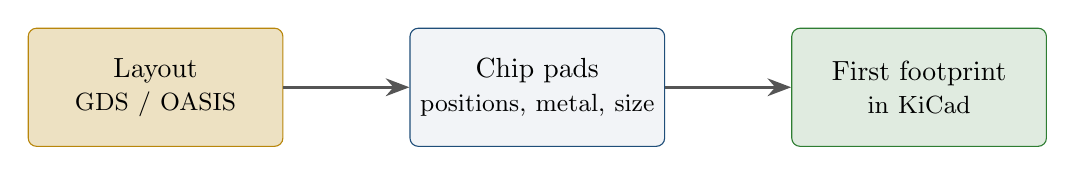
\begin{tikzpicture}[
      box/.style={draw=cobblue, rounded corners=3pt, fill=cobblue!6, align=center,
                  minimum height=1.5cm, text width=3cm},
      arr/.style={-{Stealth[length=3mm]}, very thick, color=cobgrey}]
    \node[box, fill=cobgold!25, draw=cobgold] (g) {Layout\\\small GDS / OASIS};
    \node[box, right=1.6cm of g] (c) {Chip pads\\\small positions, metal, size};
    \node[box, right=1.6cm of c, fill=cobgreen!15, draw=cobgreen] (k) {First footprint\\\small in KiCad};
    \draw[arr] (g)--(c); \draw[arr] (c)--(k);
  \end{tikzpicture}
  \vspace{0.8cm}

  \begin{itemize}\setlength\itemsep{0.6em}
    \item A tool that gives me a \textbf{first footprint} for a new chip, in minutes instead of days
    \item \textbf{Directly exported to KiCad}: symbol, footprint, no redrawing
    \item I only fix what is chip-specific. The tool does the geometry.
  \end{itemize}
\end{frame}

% ======================================================================
\begin{frame}{Step 1: extract the die from the layout (\texttt{cobgen})}
  \centering
  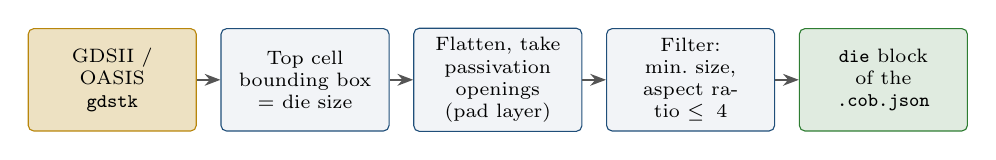
\begin{tikzpicture}[
      box/.style={draw=cobblue, rounded corners=2pt, fill=cobblue!6, align=center,
                  minimum height=1.3cm, text width=1.9cm, font=\scriptsize},
      arr/.style={-{Stealth[length=2mm]}, thick, color=cobgrey},
      node distance=0.3cm]
    \node[box, fill=cobgold!25, draw=cobgold] (a) {GDSII / OASIS\\ \texttt{gdstk}};
    \node[box, right=of a] (b) {Top cell\\ bounding box\\ $=$ die size};
    \node[box, right=of b] (c) {Flatten, take\\ passivation\\ openings\\ (pad layer)};
    \node[box, right=of c] (d) {Filter: min.\ size,\\ aspect ratio $\le 4$};
    \node[box, right=of d, fill=cobgreen!15, draw=cobgreen] (e) {\texttt{die} block\\ of the\\ \texttt{.cob.json}};
    \draw[arr] (a)--(b); \draw[arr] (b)--(c); \draw[arr] (c)--(d); \draw[arr] (d)--(e);
  \end{tikzpicture}
  \vspace{0.3cm}

  \footnotesize
  \begin{columns}[T]
    \column{0.55\textwidth}
      \begin{tabular}{@{}p{2.3cm}p{4.2cm}@{}}
        \toprule
        \textbf{Field} & \textbf{Source in the layout}\\
        \midrule
        \texttt{size} & bounding box of the top cell\\
        \texttt{center, size} & opening polygon on the pad layer\\
        \texttt{name} & text label inside the opening\\
        \texttt{electrical} & I/O cell that contains the opening\\
        \texttt{side} & nearest die edge\\
        \texttt{metal} & PDK table\\
        \bottomrule
      \end{tabular}
    \column{0.42\textwidth}
      \begin{itemize}\setlength\itemsep{0.25em}
        \item Pads numbered \texttt{D1..Dn}, counter-clockwise from bottom left
        \item Coordinates in mm, origin at the die center, Y up
        \item The PDK table is tiny: pad layer, label layer, metal, min.\ size, cell name $\to$ pin type (\texttt{gf180mcu}, \texttt{sky130})
        \item What a layout cannot know is written \texttt{"unspecified"}
      \end{itemize}
  \end{columns}
  \vfill
  {\scriptsize\color{cobgrey} Tested on the wafer.space gf180mcu example: 56 pads, 52 labeled.}
\end{frame}

% ======================================================================
\begin{frame}{Limits of the extraction, and what it takes to fix them}
  \footnotesize
  \renewcommand{\arraystretch}{1.0}
  \begin{tabular}{@{}L{2.9cm}L{3.9cm}L{5.2cm}@{}}
    \toprule
    \textbf{Limit} & \textbf{What it means} & \textbf{What it takes to fix}\\
    \midrule
    Every pad is a rectangle
      & Round or octagonal openings become boxes, so the footprint is only approximate
      & \hl{Easy, just not implemented yet.} The opening polygon is already read, it only has to be stored in the file and drawn\\
    \addlinespace[0.3em]
    One table per PDK: pad layer, label layer, I/O cell name $\to$ pin type
      & \texttt{gf180mcu} works, \texttt{sky130} is untested, other PDKs find no pads or no pin types
      & \textbf{Open PDKs:} look up the layer map, add an entry. \textbf{Closed PDKs:} layer numbers are under NDA, the chip designer must supply them (no option for that yet). Cell names need PDK knowledge\\
    \addlinespace[0.3em]
    Names and pin types are not in the layout
      & Unlabeled pads stay \texttt{"unspecified"} (4 of 56 in the example)
      & A layout has no connectivity or design intent. Name and type live in the netlist, so it needs a second input and a matching step\\
    \bottomrule
  \end{tabular}
  \vspace{0.1em}
  \begin{center}\footnotesize
    The rule: \hl{what the layout cannot know is never guessed}, it stays \texttt{"unspecified"}.
  \end{center}
\end{frame}

% ======================================================================
\begin{frame}[fragile]{Step 2: how the data is formatted in JSON}
  \footnotesize
  \begin{columns}[T]
    \column{0.45\textwidth}
      \texttt{\textbf{die}} \hl{cobgen}: chip size, notch, pads\\[0.2em]
      \texttt{\textbf{pcb}} \hl{cobedit}: shapes, pads, misc\\[0.2em]
      \texttt{\textbf{wires}} \hl{cobedit}: die pad $\to$ PCB pad, loop, bond\\[0.2em]
      \texttt{\textbf{assembly}} \hl{cobasm, not implemented yet}: die attach, bonding, tempering. Not needed for footprint and symbol.

      \vspace{0.5em}
      \textbf{Rules}
      \begin{itemize}\setlength\itemsep{0.1em}
        \item One file = one delivered die (UUID), origin at the die center, mm, Y up
        \item \texttt{"none"} = deliberately absent, \texttt{"unspecified"} = not known yet
        \item Land patterns: reusable \texttt{*.shape.cob.json}, referenced by UUID
      \end{itemize}
    \column{0.53\textwidth}
\begin{lstlisting}
"die": { "pads": [ {
  "id": "D1", "name": "CLK",
  "center": [-0.2, 0.72], "size": [0.08, 0.08],
  "metal": "Al", "side": "top",
  "electrical": "input" } ] },

"pcb": {
  "shapes": { "FINGER": "27c699bd-b041-..." },
  "pads": [ {
    "id": "P1", "number": "1", "name": "CLK",
    "shape": "FINGER", "at": [-0.4, 1.45],
    "rotation": 90, "finish": "ENIG" } ] },

"wires": { "items": [ {
  "id": "W1",
  "from": { "die_pad": "D1" },
  "to":   { "pcb_pad": "P1" },
  "type": "wedge", "diameter_um": 25,
  "loop": { "height": { "nom": 0.25,
                        "tol": 0.05 } } } ] }
\end{lstlisting}
  \end{columns}
\end{frame}

% ======================================================================
\begin{frame}[fragile]{Step 3: from JSON to a KiCad footprint (\texttt{cobkicad})}
  \centering
  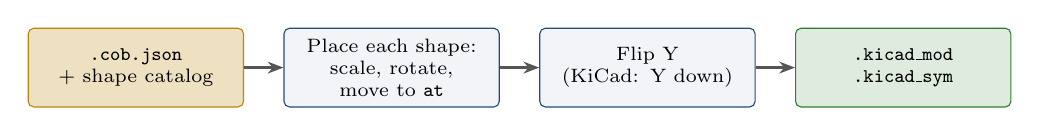
\begin{tikzpicture}[
      box/.style={draw=cobblue, rounded corners=2pt, fill=cobblue!6, align=center,
                  minimum height=1.0cm, text width=2.5cm, font=\scriptsize},
      arr/.style={-{Stealth[length=2mm]}, thick, color=cobgrey},
      node distance=0.5cm]
    \node[box, fill=cobgold!25, draw=cobgold] (a) {\texttt{.cob.json}\\ + shape catalog};
    \node[box, right=of a] (b) {Place each shape:\\ scale, rotate,\\ move to \texttt{at}};
    \node[box, right=of b] (c) {Flip Y\\ (KiCad: Y down)};
    \node[box, right=of c, fill=cobgreen!15, draw=cobgreen] (d) {\texttt{.kicad\_mod}\\ \texttt{.kicad\_sym}};
    \draw[arr] (a)--(b); \draw[arr] (b)--(c); \draw[arr] (c)--(d);
  \end{tikzpicture}
  \vspace{0.2cm}

  \footnotesize
  \begin{columns}[T]
    \column{0.58\textwidth}
      \begin{tabular}{@{}p{3.3cm}p{4.3cm}@{}}
        \toprule
        \textbf{\texttt{.cob.json}} & \textbf{KiCad}\\
        \midrule
        die outline, pads & polygons on \texttt{F.SilkS}\\
        \texttt{pcb.pads} copper & custom SMD pad on \texttt{F.Cu}\\
        \texttt{pcb.pads} mask & polygon on \texttt{F.Mask}\\
        \texttt{misc}: keepout & rule area\\
        \texttt{misc}: cutout & \texttt{Edge.Cuts}\\
        \texttt{wires.items} & lines on \texttt{Dwgs.User}\\
        die pad \texttt{electrical} & symbol pin type\\
        \bottomrule
      \end{tabular}
    \column{0.4\textwidth}
\begin{lstlisting}[basicstyle=\ttfamily\tiny]
cd tools/cobkicad
uv run cobkicad \
  --file <uuid>.cob.json \
  --out ./out
\end{lstlisting}
      \begin{itemize}\setlength\itemsep{0.2em}
        \item Writes a \texttt{.kicad\_sym} symbol library and a \texttt{.pretty} footprint library
        \item Add both as libraries in KiCad 9 or 10, place symbol and footprint
        \item One symbol pin per PCB pad, footprint carries the die, the wires and the keepouts
      \end{itemize}
  \end{columns}
\end{frame}

% ======================================================================
\begin{frame}[fragile]{How the KiCad files are written, and where this goes}
  \footnotesize
  \begin{columns}[T]
    \column{0.48\textwidth}
      \begin{block}{Today}
        s-expressions written \textbf{directly as text}, with a 25-line helper for quoting, numbers and UUIDs.\\[0.3em]
        \hl{Why:} it was the fastest way to a first footprint, and it needs no dependency.
      \end{block}
      \begin{alertblock}{Cost}
        KiCad does not check the result. The Y flip, UUIDs and layer names are spread over many format strings.
      \end{alertblock}
    \column{0.5\textwidth}
      \textbf{Next step: classes instead of strings}
\begin{lstlisting}[basicstyle=\ttfamily\scriptsize]
fp = Footprint("COB_OCJ-DEMO1")
fp.add_die(size, notch, pads)
fp.add_pad("1", "CLK",
           copper=polys, mask=mask,
           at=(-0.4, 1.45))
fp.add_keepout(poly, forbids=["via"])
fp.add_wire(die_pad, bond_target)
fp.write("open_cob.pretty")
\end{lstlisting}
      \begin{itemize}\setlength\itemsep{0.15em}
        \item Thin classes (\texttt{Footprint}, \texttt{Symbol}), each item knows how to become an s-expression tree
        \item One serializer, one place for the Y flip and UUIDs
        \item Same idea for symbols: \texttt{add\_pin()}
        \item The writer behind the classes can change later, for example to an s-expression library
      \end{itemize}
  \end{columns}
\end{frame}

% ======================================================================
\begin{frame}{What does the open.cob workflow already do?}
  \begin{columns}[T]
    \column{0.48\textwidth}
      \begin{description}\setlength\itemsep{0.35em}
        \item[\texttt{cobtestdata}] fetches the manufactured wafer.space reticles as test input
        \item[\texttt{cobgen}] GDSII / OASIS $\to$ \texttt{die} block
        \item[\texttt{cobedit}] place PCB pads from a shape catalog, add wires
        \item[\texttt{cobviz}] render the bonding plan as SVG
        \item[\texttt{cobkicad}] KiCad 9/10 symbol and footprint
      \end{description}
      \vspace{0.4em}
      \small Work in progress. \texttt{cobasm} (assembly) is not implemented yet.\\
      {\scriptsize\texttt{github.com/MaxClerkwell/open.cob.json}}
    \column{0.5\textwidth}
      \centering
      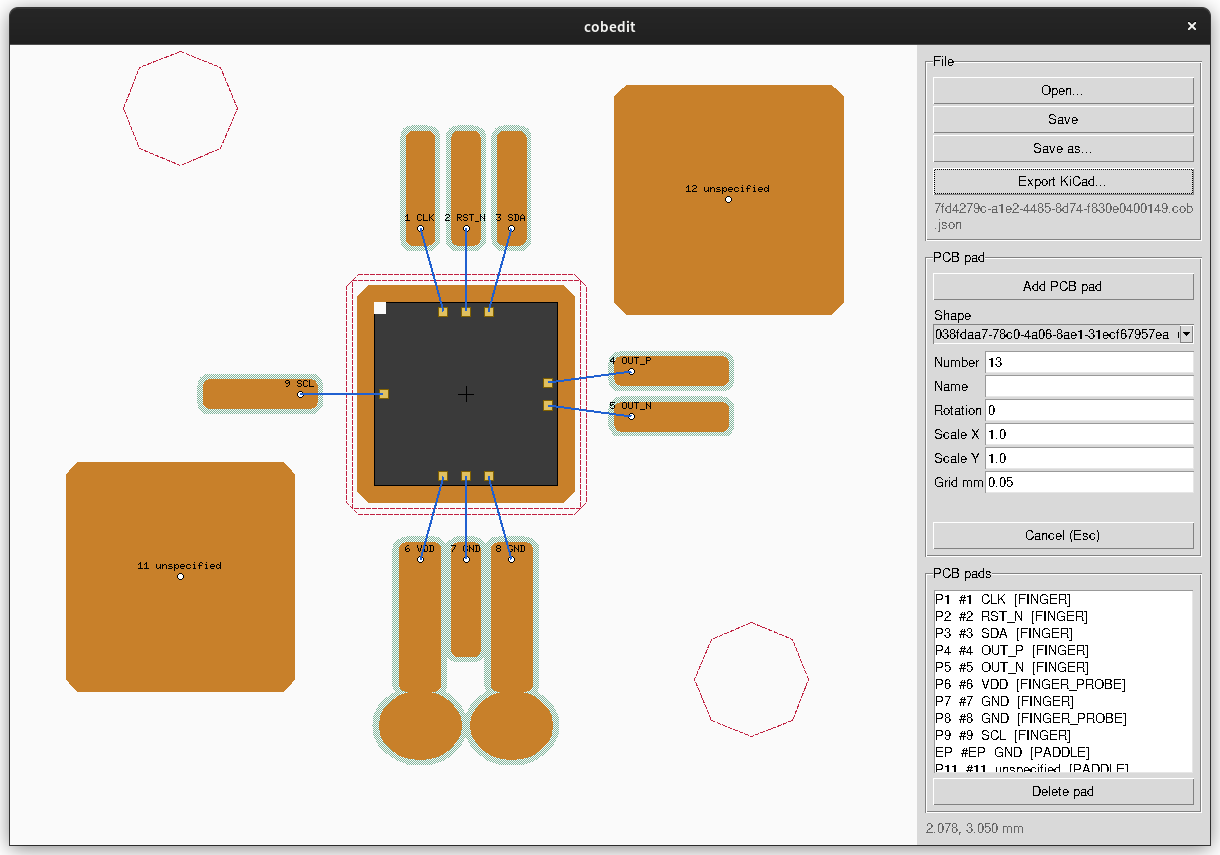
\includegraphics[width=\textwidth]{images/cobedit-screenshot.png}\\[0.2em]
      {\scriptsize\color{cobgrey} \texttt{cobedit} with the fictional demo chip}
  \end{columns}
\end{frame}

% ======================================================================
\begin{frame}{Why not a KiCad plugin?}
  \footnotesize
  \begin{columns}[T]
    \column{0.47\textwidth}
      \begin{alertblock}{A plugin makes KiCad a dependency}
        \begin{itemize}\setlength\itemsep{0.15em}
          \item The workflow lives inside one tool and follows its versions and its API
          \item Only KiCad users can use it
          \item The chip designer would have to know the PCB designer's EDA
        \end{itemize}
      \end{alertblock}
      \begin{exampleblock}{Open format plus generator}
        \begin{itemize}\setlength\itemsep{0.15em}
          \item Nothing depends on KiCad, it is one output among others
          \item Other EDA tools can adopt the format
          \item The chip designer delivers one file, whatever the board is designed in
        \end{itemize}
      \end{exampleblock}
    \column{0.5\textwidth}
      \centering
      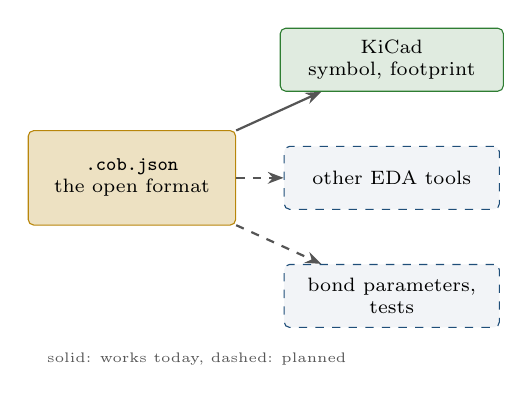
\begin{tikzpicture}[
          box/.style={draw=cobblue, rounded corners=2pt, fill=cobblue!6, align=center,
                      minimum height=0.8cm, text width=2.6cm, font=\scriptsize},
          done/.style={box, fill=cobgreen!15, draw=cobgreen},
          plan/.style={box, dashed, text width=2.5cm},
          arr/.style={-{Stealth[length=2mm]}, thick, color=cobgrey},
          parr/.style={-{Stealth[length=2mm]}, thick, dashed, color=cobgrey}]
        \node[box, fill=cobgold!25, draw=cobgold, text width=2.4cm, minimum height=1.2cm] (c) at (0,0) {\texttt{.cob.json}\\ the open format};
        \node[done] (k) at (3.3,1.5) {KiCad\\ symbol, footprint};
        \node[plan] (e) at (3.3,0) {other EDA tools};
        \node[plan] (t) at (3.3,-1.5) {bond parameters,\\ tests};
        \draw[arr] (c)--(k); \draw[parr] (c)--(e); \draw[parr] (c)--(t);
        \node[font=\tiny, color=cobgrey, anchor=west] at (-1.2,-2.3) {solid: works today, dashed: planned};
      \end{tikzpicture}
  \end{columns}
\end{frame}

% ======================================================================
\begin{frame}[fragile]{Demo: from the reticle to the footprint}
\begin{lstlisting}[language=cobshell, basicstyle=\ttfamily\scriptsize, commentstyle=\color{cobblue}\bfseries]
# 1. Initialize: fetch the shuttle reticle and manifest, once
uv run initialize_testdata --run 2

# 2. Pick a chip from the menu (one folder per chip)
uv run extract_die --run 2

# 3. Extract the die from the layout into a .cob.json
uv run cobgen --file testdata/dies/CAFE/chip_top.oas \
              --pdk gf180mcu --out testdata/dies/CAFE/CAFE.cob.json

# 4. Add PCB pads and wires in the editor
uv run cobedit --file testdata/dies/CAFE/CAFE.cob.json

# 5. Generate symbol and footprint
uv run cobkicad --file testdata/dies/CAFE/CAFE.cob.json \
                --out testdata/dies/CAFE/kicad

# 6. KiCad: add the .kicad_sym and the .pretty folder as
#    libraries, place the symbol
\end{lstlisting}
\end{frame}

% ======================================================================
\begin{frame}{Next steps}
  \begin{enumerate}\setlength\itemsep{0.55em}
    \item Check with a design service and a bonding service whether I overlooked important points that need another look
    \item Test more chips, to find what I overlooked
    \item Integrate other PDKs
    \item Find a workaround or a fix for pads with multiple labels
    \item Add automatic wire shape generation
    \item Improve the shape catalog in \texttt{cobedit}
  \end{enumerate}
  \vfill
  \begin{center}\small\color{cobgrey}
    And one completely different approach: glue the die and connect it with a flex PCB (next slide).
  \end{center}
\end{frame}

% ======================================================================
\begin{frame}{A different approach: glue plus flex PCB}
  \small
  \begin{columns}[T]
    \column{0.5\textwidth}
      \centering
      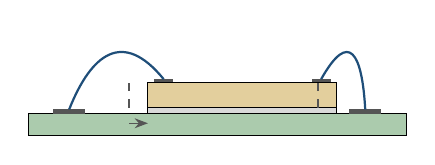
\begin{tikzpicture}[scale=0.8]
        \draw[fill=cobgreen!40] (0,0) rectangle (6,0.35);
        \fill[cobgrey] (0.4,0.35) rectangle (0.9,0.42); \fill[cobgrey] (5.1,0.35) rectangle (5.6,0.42);
        \draw[fill=black!15] (1.9,0.35) rectangle (4.9,0.45);
        \draw[fill=cobgold!40] (1.9,0.45) rectangle (4.9,0.85);
        \fill[cobgrey] (2.0,0.85) rectangle (2.3,0.9); \fill[cobgrey] (4.5,0.85) rectangle (4.8,0.9);
        \draw[thick, cobblue] (2.15,0.9) .. controls (1.5,1.7) and (1.0,1.3) .. (0.65,0.42);
        \draw[thick, cobblue] (4.65,0.9) .. controls (5.1,1.7) and (5.3,1.3) .. (5.35,0.42);
        \draw[dashed, cobgrey] (1.6,0.45) -- (1.6,0.85); \draw[dashed, cobgrey] (4.6,0.45) -- (4.6,0.85);
        \draw[-{Stealth}, cobgrey] (1.6,0.2) -- (1.9,0.2);
      \end{tikzpicture}\\[0.1em]
      \textbf{Wire bonding}: the die sits off by a bit, each wire still lands on its pad
    \column{0.5\textwidth}
      \centering
      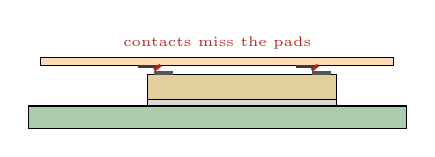
\begin{tikzpicture}[scale=0.8]
        \draw[fill=cobgreen!40] (0,0) rectangle (6,0.35);
        \draw[fill=black!15] (1.9,0.35) rectangle (4.9,0.45);
        \draw[fill=cobgold!40] (1.9,0.45) rectangle (4.9,0.85);
        \fill[cobgrey] (2.0,0.85) rectangle (2.3,0.9); \fill[cobgrey] (4.5,0.85) rectangle (4.8,0.9);
        \draw[fill=orange!30] (0.2,1.0) rectangle (5.8,1.12);
        \fill[cobgrey!70!black] (1.75,1.0) rectangle (2.05,0.96); \fill[cobgrey!70!black] (4.25,1.0) rectangle (4.55,0.96);
        \draw[cobred, very thick] (2.0,0.92) -- (2.1,1.0); \draw[cobred, very thick] (4.5,0.92) -- (4.6,1.0);
        \node[font=\tiny, color=cobred] at (3.0,1.35) {contacts miss the pads};
      \end{tikzpicture}\\[0.1em]
      \textbf{Flex PCB}: the pattern is fixed, a shifted die misaligns every contact at once
  \end{columns}
  \vspace{0.6em}
  \begin{itemize}\setlength\itemsep{0.3em}
    \item The idea: glue the die and connect it with a flex PCB instead of wires
    \item Open questions about the tolerances, to be evaluated experimentally
    \item Wires compensate tolerances better than a flex PCB, especially when the die shifts during placement
  \end{itemize}
\end{frame}

% ======================================================================
\begin{frame}{About me - Stephan Bökelmann}
  \setlength{\stackw}{0.7\textwidth}
  \newcommand{\aboutstack}{%
    \begin{minipage}[t]{\stackw}
      \footnotesize
      \begin{beamercolorbox}[wd=\linewidth,sep=0.4em]{block title alerted}
        Scientific Research Engineer at Facility for Antiproton and Ion Research
      \end{beamercolorbox}
      \vspace{0.2em}
      \begin{beamercolorbox}[wd=\linewidth,sep=0.4em]{block title alerted}
        Newest startup: \textbf{skAInet}
      \end{beamercolorbox}
      \vspace{0.2em}
      \begin{beamercolorbox}[wd=\linewidth,sep=0.4em]{block title alerted}
        \textbf{Hire me and my team via nabla B engineering}
      \end{beamercolorbox}
      \vspace{0.2em}
      \begin{beamercolorbox}[wd=\linewidth,sep=0.4em]{block title alerted}
        \textbf{Follow me} for digital design, physics and ASICs\\[0.3em]
        \scriptsize
        \faGlobe\ maxclerkwell.tech \quad \faInstagram\ Instagram \quad \xhslogo\ Xiaohongshu \quad \faDiscord\ Discord
      \end{beamercolorbox}
    \end{minipage}}
  \sbox{\stackbox}{\aboutstack}
  \setlength{\stackh}{\dimexpr\ht\stackbox+\dp\stackbox\relax}
  \noindent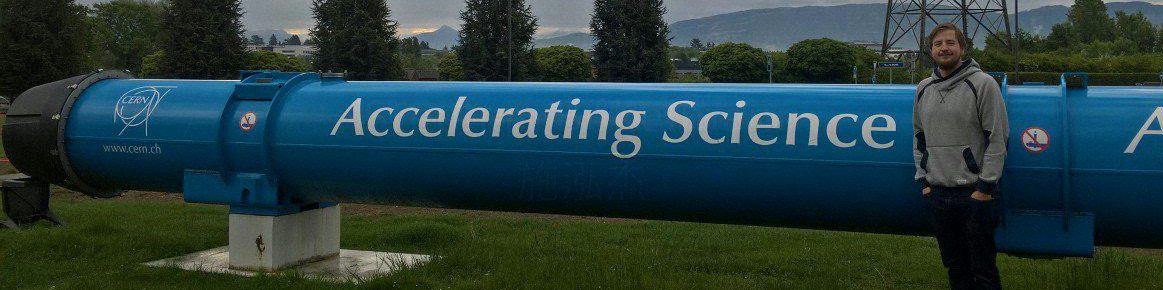
\includegraphics[width=\textwidth]{images/portrait-cern.jpg}
  \vfill
  \begin{columns}[T,onlytextwidth]
    \column{\stackw}
      \aboutstack
    \column{\stackh}
      \qrcode[tight,height=\stackh]{https://nabla-b.engineering/en/business-card/}
  \end{columns}
\end{frame}

\end{document}
